\begin{center}
    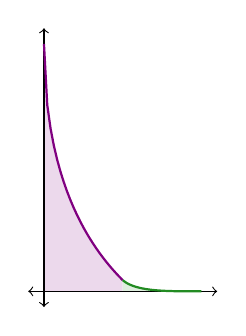
\begin{tikzpicture}
        \fill[color=Purple!15, thick, domain=0:1] plot (\x, {pi - 4 * sqrt(\x) + \x}) -- (1, 0) -- (0, 0) -- cycle;
        \fill[color=ForestGreen!15, thick, domain=1:2] plot (\x, {pi - \x - 2 - 4 * rad(atan(sqrt(\x - 1))) + 4 * sqrt(\x - 1)}) -- (1, 0) -- cycle;

        \draw[<->] (-0.2, 0) -- (2.2, 0);
        \draw[<->] (0, -0.2) -- (0, 3.3415);

        \draw[color=Purple, thick, domain=0:1] plot (\x, {pi - 4 * sqrt(\x) + \x});
        \draw[color=ForestGreen, thick, domain=1:2] plot (\x, {pi - \x - 2 - 4 * rad(atan(sqrt(\x - 1))) + 4 * sqrt(\x - 1)});
    \end{tikzpicture}
\end{center}
\captionof{figure}{The distribution of the squared distances. It looks rather odd in a way, and the presence of \( \pi \) terms seems quite interesting.}
